\documentclass[12pt]{article} 
\usepackage{amsmath} 
\usepackage{amsfonts}
\usepackage{amssymb} 
\usepackage[utf8]{inputenc} 
\usepackage[T1,T2A]{fontenc}
\usepackage[english, russian]{babel} 
\usepackage{graphicx}
\usepackage{float}
\usepackage[left=2cm,right=2cm,top=2cm,bottom=2cm]{geometry}
\usepackage{wrapfig} 
\usepackage{setspace} 
\usepackage{indentfirst}
\usepackage{subfigure} 
\usepackage[table,xcdraw]{xcolor}

\title{ 
Лабораторная работа 2.1.3 \\ <<Определение $C_P/C_V$ по скорости звука в
газе>> 
}

\author{Балдин Виктор, Б01-303}

\begin{document} 
\maketitle

\paragraph{Цель работы:} 1) измерение частоты колебаний и длины волны при
резонансе звуковых колебаний в газе, заполняющем трубу; 2) определение
показателя адиабаты с помощью уравнения состояния идеального газа.  
\paragraph{В работе используются:} звуковой генератор ГЗ; электорнный 
осциллограф ЭО, микрофон; телефон; раздвижная труба; теплоизолированная труба, 
обогреваемая водой из термостата; баллон со сжатым углекислым газом; 
газгольдер.

\section{Теоретическая справка} Один из наиболее точных методов измерения
показателя адиабаты $\gamma$ основан на зависимости от него скорости
распространения звуковой волны в газе. Последняя в газах определяется формулой
$c = \sqrt{\frac{\gamma RT}{\mu}}$, из которой можно выразить показатель
адиабаты: 
\begin{equation} 
\gamma = \frac{\mu}{RT}c^2, 
\end{equation} где $T$
--- температура газа, $\mu$ --- его молярная масса, а $R$ --- газовая
постоянная. \\ Скорость $c$ звука связана с его частотой $f$ и длиной волны
$\lambda$ соотношением 
\begin{equation} 
c = \lambda f
\end{equation} 
С волнами
в трубке удобнее всего работать при резонансе. Условие резонанса выглядит как
\begin{equation} 
L = n\frac{\lambda}{2}
\end{equation} где $L$ --- длина
трубки, $\lambda$ --- длина волны, $n$ --- целое число.\\ В данной работе при
постоянной длине трубки изменяется частота звуковых колебаний $f$, а с ней и
длина звуковой волны $\lambda$. Для последовательных резонансов можно записать:
\begin{equation} 
L = n\frac{\lambda_1}{2} = (n + 1)\frac{\lambda_2}{2} = ... =
(n + k)\frac{\lambda_{k + 1}}{2} 
\end{equation} 
С учётом (2) имеем
\begin{equation} 
f_{t+1} = \frac{c}{\lambda_{t+1}} = f_1 + \frac{c}{2L}t~ (t =
0, 1,..., k) 
\end{equation} 
Таким образом, $c/2L$ можно найти как угловой
коэффициент графика зависимости частоты от номера резонанса.
\subsection*{Экспериментальная установка} Схема установки, используемой в работе
приведена на рис. 1.\\ 
\begin{figure}[H] 
\centering
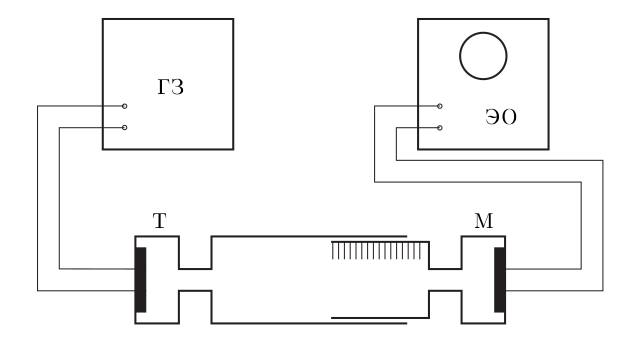
\includegraphics[scale=2]{stand.png} 
\caption{Схема установки}
\end{figure} 
Звуковые колебания в трубе возбуждаются телефоном Т и улавливаются
микрофоном М. Мембрана телефона приводится в движение переменным током звуковой
частоты.  В качестве источника переменной ЭДС используется звуковой генератор
ГЗ. Возникающий в микрофоне сигнал возникает на экране осциллографа ЭО. \\
Микрофон и телефон присоединены к установке через тонкие резиновые трубки. Такая
связь достаточна для возбуждения и обнаружения звуковых колебаний в трубе и в то
же время мало возмущает эти колебания: при расчетах оба конца трубы можно
считать неподвижными, а влиянием соединительных отверстий пренебречь. \\
Установка содерджит теплоизолированную трубу постоянной длины. Воздух в трубке
нагревается водой из термостата. Температура газа принимается равной температуре
омывающей трубу воды. 

\section{Ход работы}
\end{document}
